\documentclass[11pt]{article}
\usepackage[margin=0.7in]{geometry}
\usepackage[T1]{fontenc}
\IfFileExists{lmodern.sty}{\usepackage{lmodern}}{}
\usepackage{amsmath}
\usepackage{booktabs}
\usepackage{graphicx}
\usepackage{float}
\usepackage{caption}
\usepackage{subcaption}
\usepackage{enumitem}
\usepackage{xcolor}
\usepackage[compact]{titlesec}
\usepackage{hyperref}
\usepackage{pgfplots}
\pgfplotsset{compat=1.17}
\hypersetup{colorlinks=true, linkcolor=blue!50!black, citecolor=blue!50!black, urlcolor=blue!50!black}
\captionsetup{font=small, labelfont=bf, skip=3pt}
\setlist{nosep, leftmargin=*}
\setlength{\parskip}{3pt}
\setlength{\parindent}{0pt}
\setlength{\textfloatsep}{8pt}
\setlength{\floatsep}{6pt}
\setlength{\intextsep}{6pt}
\titlespacing*{\section}{0pt}{6pt}{3pt}
\titlespacing*{\subsection}{0pt}{4pt}{2pt}
\titlespacing*{\paragraph}{0pt}{2pt}{0.6em}
\renewcommand{\refname}{References}

\newcommand{\code}[1]{\texttt{#1}}

\pgfplotsset{
  rpt/.style={
    height=4.6cm,
    grid=major, grid style={gray!20},
    tick label style={font=\scriptsize}, label style={font=\footnotesize},
    legend style={font=\scriptsize, row sep=-2pt, inner sep=1pt},
  }
}

\title{\vspace{-2.5em}CSE 256 Fall 2026: PA2 Report\\
\large Part A: Transformer Encoder and Decoder (Parts 1--2)}
\author{Garvit Gopalani}
\date{}

\begin{document}
\maketitle
\vspace{-3.2em}

\begin{center}
\small Sections follow the Gradescope rubric: 1.1--1.5 and 2.1--2.4 are below. Rubric items 3--5 (Part 3) are in the executed notebook attached as Part B; see the map on the last page of Part A.
\end{center}

%=====================================================================
\section*{1\quad Part 1: Encoder Trained With a Classifier}
%=====================================================================

\subsection*{1.1\quad Encoder Implementation}

Following Vaswani et al.~\cite{vaswani} and Karpathy's tutorial~\cite{karpathy}, \code{transformer.py} implements the encoder from scratch, using only \code{nn.Linear}, \code{nn.Embedding} and \code{nn.LayerNorm} (no library Transformer or attention layers).

\begin{itemize}
  \item \textbf{Input.} Word ids come from the provided NLTK word-level tokenizer (5{,}634 types, built from the two training files). Each id gets a token embedding plus a learned absolute position embedding (block size 32); the two are added before the first block.
  \item \textbf{Blocks.} $N=4$ Transformer blocks with pre-LayerNorm and a residual connection around each sub-layer:
  \begin{itemize}
    \item \emph{Multi-head self-attention:} 2 heads of size 32. Each head computes $\mathrm{softmax}(QK^\top/\sqrt{32})\,V$; the head outputs are concatenated and projected back to 64 dimensions.
    \item \emph{Feedforward layer:} $64 \rightarrow 100 \rightarrow 64$ with ReLU.
  \end{itemize}
  \item \textbf{Output.} A final LayerNorm gives one 64-dimensional contextual vector per input word. The encoder also returns every attention map (one per head per layer) for the sanity checks.
  \item \textbf{Padding.} Segments are truncated or padded to 32 tokens with \code{<pad>} (id 0). Padding positions are masked as attention keys (score $-\infty$ before the softmax), so every row of a map is a distribution over the real words only.
  \item \textbf{Initialization.} Weights from $\mathcal{N}(0, 0.02)$, zero biases (GPT-2 style).
\end{itemize}

\textbf{Number of parameters in the encoder: 481{,}424.} Token embeddings $5{,}634 \times 64 = 360{,}576$; position embeddings 2{,}048; four blocks of 29{,}668 each ($Q$, $K$, $V$ 12{,}288; output projection 4{,}160; feedforward 12{,}964; two LayerNorms 256); final LayerNorm 128.

\subsection*{1.2\quad Feedforward Classifier Implementation}

\code{FeedForwardClassifier} and \code{EncoderClassifier} in \code{transformer.py}:
\begin{itemize}
  \item \textbf{Summary vector.} The encoder outputs are averaged over the sequence. Only the real (non-padding) positions count: $\bar{h} = \frac{1}{n}\sum_{i=1}^{n} h_i$, where $n$ is the segment's length.
  \item \textbf{Classifier.} A feedforward network with one hidden layer, $64 \rightarrow 100 \rightarrow 3$ with ReLU (sizes from \code{main.py}), maps $\bar{h}$ to one score per speaker (0 Obama, 1 W.\ Bush, 2 H.\ W.\ Bush).
  \item \textbf{Parameters.} The classifier has 6{,}803 parameters ($64 \times 100 + 100$ and $100 \times 3 + 3$), for 488{,}227 in total with the encoder.
\end{itemize}

\subsection*{1.3\quad Joint Encoder \& Classifier Training}

\begin{itemize}
  \item \textbf{One model, one optimizer.} Encoder and classifier form a single model trained jointly from scratch, with no pretraining. Each batch of 16 segments goes through the encoder and the classifier. The cross-entropy loss against the true speaker is backpropagated through both, and one Adam optimizer (learning rate $10^{-3}$) updates all parameters.
  \item \textbf{Schedule.} 15 epochs over the 2{,}092 training segments, reshuffled every epoch. After each epoch, train and test accuracy are computed with the model in evaluation mode. Training takes about 100\,s on my laptop CPU (\code{python main.py part1}).
  \item \textbf{Reproducibility.} I made the tokenizer assign ids in sorted order: iterating over a Python set of strings depends on the hash seed, so ids changed between runs. A fixed seed now gives identical results on the same machine. Different PyTorch builds or CPUs still give slightly different numbers.
\end{itemize}

To see which training choices matter, I repeated the run with three more seeds, without the padding mask (\code{--no\_pad\_mask}), and with PyTorch's default initialization (\code{--init default}). Table~\ref{tab:seeds1} shows the results.

\begin{table}[H]
\centering
\footnotesize
\setlength{\tabcolsep}{5pt}
\caption{Test accuracy (\%) over four seeds (42, 1, 2, 3) with and without masking padding, and with PyTorch's default initialization (seed 42). Mean $\pm$ standard deviation over seeds; the epoch 1 and 5 columns are means.}
\label{tab:seeds1}
\begin{tabular}{@{}l c l c c@{}}
\toprule
Setting & Final (ep.\ 15) & Per seed & Ep.\ 1 & Ep.\ 5 \\
\midrule
Padding masked (default) & 87.5 $\pm$ 1.4 & 87.33, 89.47, 86.13, 87.20 & \textbf{54.2} & \textbf{85.8} \\
Padding not masked & 87.7 $\pm$ 0.4 & 88.00, 87.07, 87.73, 88.00 & 38.9 & 80.2 \\
PyTorch default init & 85.9 & --- & 42.7 & 73.5 \\
\bottomrule
\end{tabular}
\end{table}

\begin{itemize}
  \item \textbf{Masking padding speeds up early training but does not change the final accuracy.} Without the mask, every word attends to up to 31 padding positions, and the mean includes them. The final accuracy is the same within noise ($87.7 \pm 0.4\%$ vs $87.5 \pm 1.4\%$), but early training is much slower without the mask:
  \begin{itemize}
    \item after epoch 1, two of four unmasked runs are still at chance (33.3\%), and the mean is 38.9\% vs 54.2\%;
    \item one unmasked run is only at 61.3\% after epoch 5 and needs until epoch 8 to pass 80\%.
  \end{itemize}
  The unmasked model must first learn to ignore a large, length-dependent share of identical padding vectors. Masking removes that problem.
  \item \textbf{Initialization mostly changes the speed.} With PyTorch's default initialization ($\mathcal{N}(0,1)$ embeddings), the model learns more slowly (73.5\% vs 86.4\% at epoch 5). It ends at 85.9\%, 1.4 points lower, which is within seed noise (Figure~\ref{fig:p1}, dotted line).
\end{itemize}

\subsection*{1.4\quad Sanity Checks}

\textbf{Rows sum to 1.} The \code{utilities.py} check passes for both test sentences: every row of all 8 attention maps (4 layers $\times$ 2 heads) sums to 1.

\textbf{Attention maps.} Figure~\ref{fig:attn-enc} shows all eight maps for one Obama sentence (row = query word, column = key word). To check that the picture holds beyond one sentence, \code{main.py} also prints statistics for every head, averaged over the 750 test segments (Table~\ref{tab:attn}).

\begin{figure}[H]
\centering
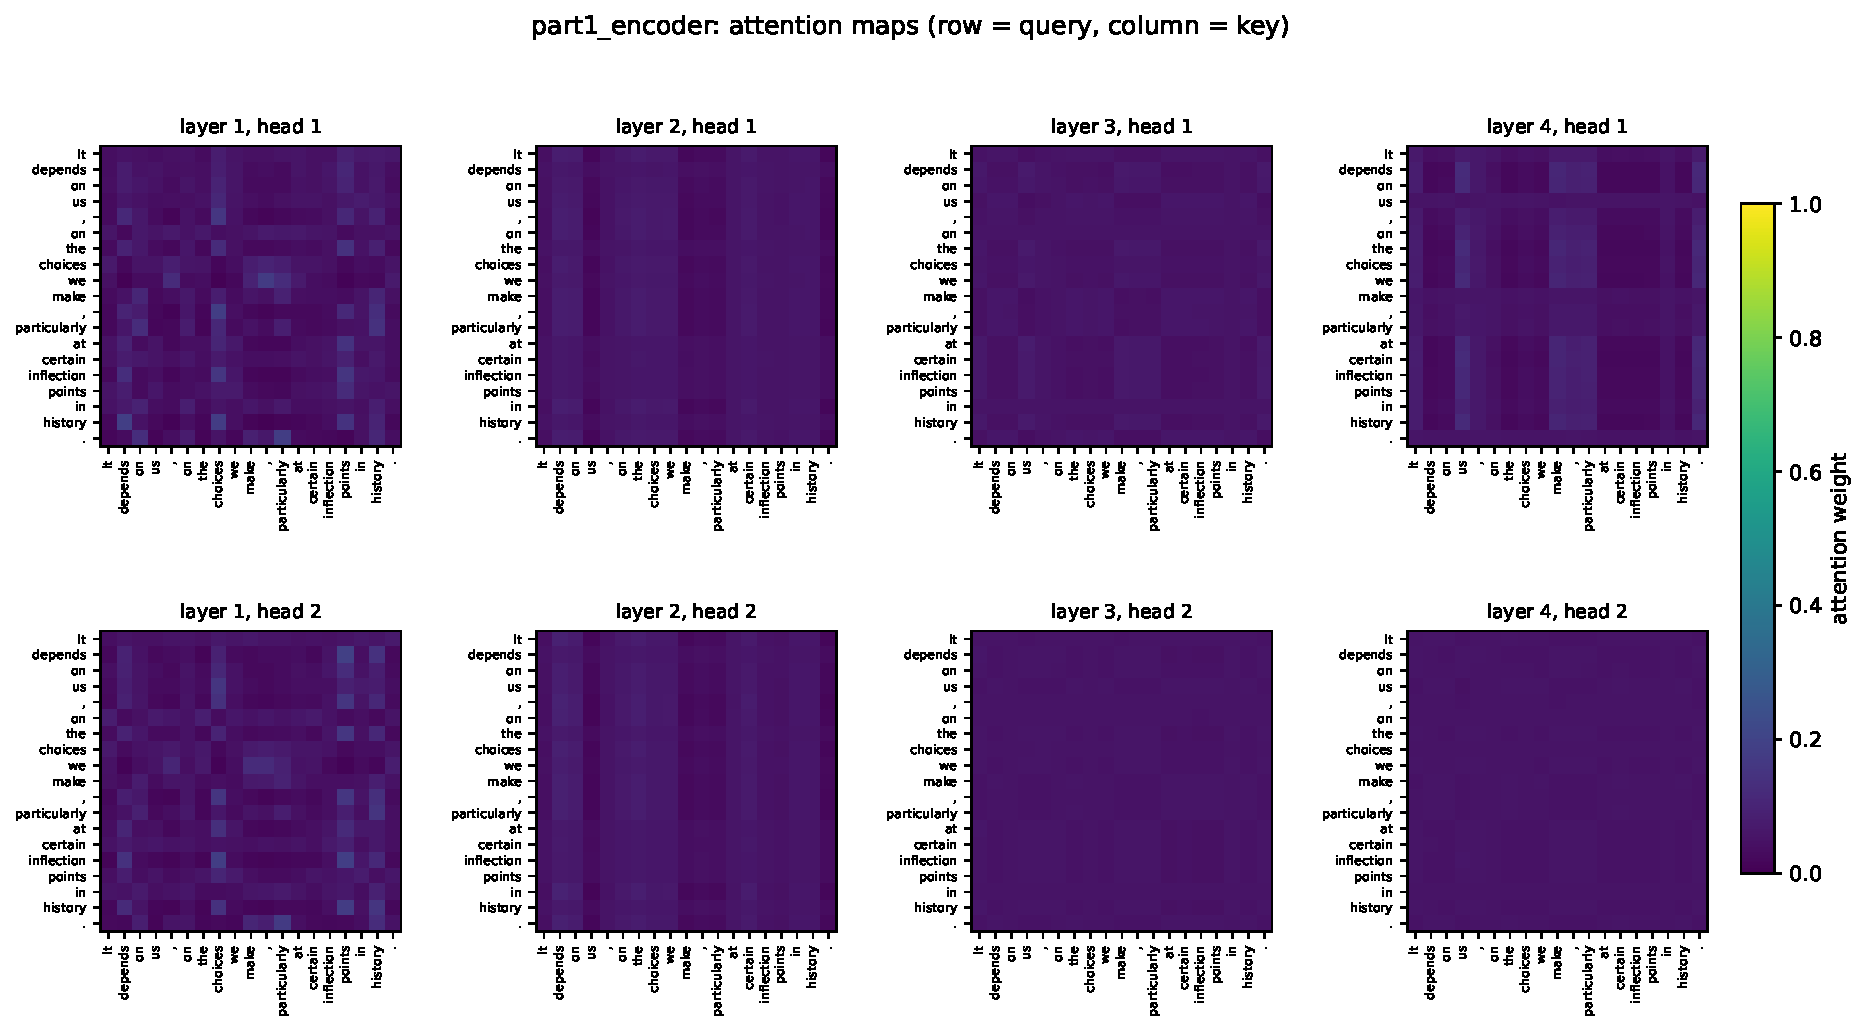
\includegraphics[width=0.82\linewidth, trim=0 0 0 40, clip]{figures/part1_encoder_attention_s1.pdf}
\caption{Encoder attention maps for ``It depends on us, on the choices we make, particularly at certain inflection points in history.'' Rows are heads, columns are layers. Each row of a map is one query word's distribution over the key words.}
\label{fig:attn-enc}
\end{figure}

\begin{table}[H]
\centering
\footnotesize
\setlength{\tabcolsep}{4pt}
\caption{Attention statistics per head: encoder averaged over the test segments; decoder (Section~2.3) over \code{test\_LM\_obama.txt}, first position of each window excluded. Entropy is divided by $\log(\#\text{visible keys})$, so 1 = uniform. Max = largest weight in a row. Self / Previous = weight on the query's own / previous position.}
\label{tab:attn}
\begin{tabular}{@{}c ccc c cccc@{}}
\toprule
& \multicolumn{3}{c}{Encoder (Part 1)} && \multicolumn{4}{c}{Decoder (Part 2)} \\
\cmidrule{2-4}\cmidrule{6-9}
Layer.head & Entropy & Max & Self && Entropy & Max & Self & Previous \\
\midrule
1.1 & 0.941 & 0.138 & 0.055 && 0.967 & 0.161 & 0.077 & \textbf{0.113} \\
1.2 & \textbf{0.939} & \textbf{0.141} & 0.057 && 0.977 & 0.149 & 0.088 & 0.107 \\
2.1 & 0.978 & 0.086 & 0.055 && 0.985 & 0.138 & 0.089 & 0.102 \\
2.2 & 0.975 & 0.089 & 0.056 && 0.939 & \textbf{0.197} & 0.097 & 0.106 \\
3.1 & 0.997 & 0.067 & 0.052 && \textbf{0.928} & 0.196 & \textbf{0.110} & 0.096 \\
3.2 & 1.000 & 0.057 & 0.054 && 0.978 & 0.147 & 0.095 & 0.101 \\
4.1 & 0.976 & 0.099 & 0.048 && 0.970 & 0.159 & 0.097 & 0.099 \\
4.2 & 1.000 & 0.058 & 0.054 && 0.988 & 0.133 & 0.093 & 0.101 \\
\midrule
Uniform & 1 & 0.054 & 0.054 && 1 & 0.099 & 0.099 & 0.099 \\
\bottomrule
\end{tabular}
\end{table}

\textbf{What the encoder maps show.}
\begin{itemize}
  \item \textbf{Most heads simply average over the sentence.} Every encoder head has normalized entropy between 0.939 and 1.000. Head 2 in layers 3 and 4 is uniform to three decimals: entropy 1.000, and a largest weight of 0.057--0.058 against 0.054 for uniform attention. These heads just mix the whole sentence into every position.
  \item \textbf{The little structure there is sits in the first layer and depends on the key.}
  \begin{itemize}
    \item The two layer-1 heads are the most selective, with entropy 0.94 and a largest weight of about 0.14, 2.6 times uniform.
    \item In Figure~\ref{fig:attn-enc} their structure is mostly faint vertical stripes: a few content words, such as \textit{choices}, \textit{points} and \textit{history}, get slightly more attention from every position.
    \item Layer 4 head 1 (entropy 0.976) shows similar stripes.
  \end{itemize}
  \item \textbf{No preference for the word itself.} The weight on the query's own position (0.048--0.057) is about what uniform attention gives (0.054).
  \item \textbf{This fits the training signal.} The classifier only sees the mean over positions, so nothing pushes the encoder toward sharp, position-specific attention. Near-uniform heads mix each word's information into every position, which is exactly what the mean then reads. The second sanity sentence (\code{part1\_encoder\_attention\_s2.png}) looks the same.
\end{itemize}

\subsection*{1.5\quad Evaluation}

Table~\ref{tab:p1} and Figure~\ref{fig:p1} give the test accuracy on \code{test\_CLS.tsv} after each of the 15 epochs (seed 42). The \textbf{final test accuracy is 87.33\%} (best 87.60\%, at epoch 9), slightly above the expected low-to-mid 80s. The encoder has 481{,}424 parameters (Section~1.1).

\begin{table}[H]
\centering
\footnotesize
\setlength{\tabcolsep}{3.2pt}
\caption{Part 1, seed 42: training loss, train accuracy and test accuracy (\%) after each epoch.}
\label{tab:p1}
\begin{tabular}{@{}l *{15}{c}@{}}
\toprule
Epoch & 1 & 2 & 3 & 4 & 5 & 6 & 7 & 8 & 9 & 10 & 11 & 12 & 13 & 14 & 15 \\
\midrule
Train loss & 1.037 & .798 & .604 & .454 & .266 & .117 & .055 & .031 & .033 & .044 & .018 & .012 & .010 & .014 & .010 \\
Train acc  & 62.6 & 72.0 & 79.7 & 89.9 & 96.9 & 98.7 & 99.4 & 99.2 & 98.8 & 99.3 & 99.6 & 99.7 & 99.8 & 99.7 & 99.8 \\
Test acc   & 53.2 & 61.3 & 68.5 & 77.5 & 86.4 & 85.6 & 86.9 & 86.4 & \textbf{87.6} & 85.9 & 86.9 & 87.5 & 86.8 & 87.1 & \textbf{87.3} \\
\bottomrule
\end{tabular}
\end{table}

\begin{figure}[H]
\centering
\begin{minipage}[c]{0.42\linewidth}
\centering
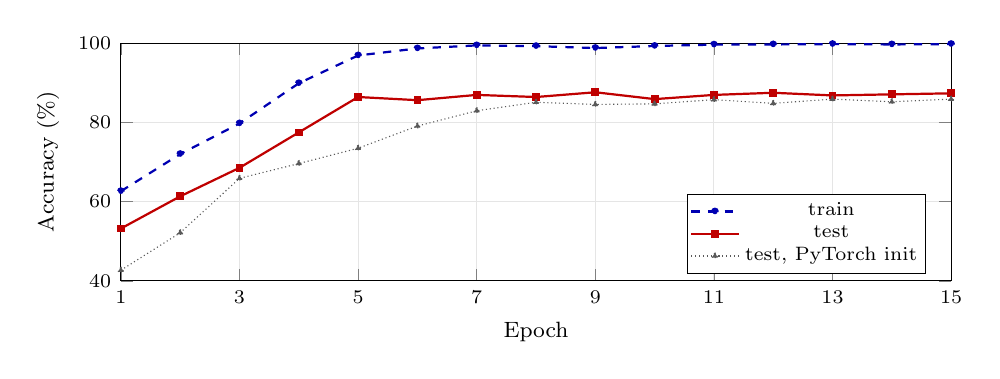
\begin{tikzpicture}
\begin{axis}[rpt, width=\linewidth,
  xlabel={Epoch}, ylabel={Accuracy (\%)},
  xmin=1, xmax=15, ymin=40, ymax=100, xtick={1,3,5,7,9,11,13,15},
  legend pos=south east]
\addplot[thick, dashed, color=blue!70!black, mark=*, mark size=1pt] coordinates {
(1,62.62)(2,71.99)(3,79.73)(4,89.87)(5,96.89)(6,98.66)(7,99.43)(8,99.24)(9,98.76)(10,99.28)(11,99.62)(12,99.67)(13,99.76)(14,99.67)(15,99.76)};
\addlegendentry{train}
\addplot[thick, color=red!75!black, mark=square*, mark size=1pt] coordinates {
(1,53.20)(2,61.33)(3,68.53)(4,77.47)(5,86.40)(6,85.60)(7,86.93)(8,86.40)(9,87.60)(10,85.87)(11,86.93)(12,87.47)(13,86.80)(14,87.07)(15,87.33)};
\addlegendentry{test}
\addplot[thin, densely dotted, color=gray!70!black, mark=triangle*, mark size=1.2pt] coordinates {
(1,42.67)(2,52.13)(3,65.87)(4,69.60)(5,73.47)(6,79.07)(7,82.93)(8,85.07)(9,84.53)(10,84.67)(11,85.73)(12,84.80)(13,85.87)(14,85.20)(15,85.87)};
\addlegendentry{test, PyTorch init}
\end{axis}
\end{tikzpicture}
\captionof{figure}{Part 1 accuracy by epoch (seed 42).}
\label{fig:p1}
\end{minipage}\hfill
\begin{minipage}[c]{0.54\linewidth}
\textbf{Discussion.}
\begin{itemize}
  \item \textbf{Fast learning, then a plateau.} Test accuracy jumps from 77\% to 86\% at epoch 5, the same epoch train accuracy jumps from 90\% to 97\%. From epoch 5 on, test accuracy stays between 85.6\% and 87.6\% while the training loss keeps falling toward 0.
  \item \textbf{The model overfits, but test accuracy holds.} From epoch 6 on it fits the training set almost perfectly (98.7--99.8\%), with about 488K parameters for 2{,}092 segments. Test accuracy stops improving but does not drop.
\end{itemize}
\end{minipage}
\end{figure}

\textbf{Single runs are noisy by 1--3 points.} Over four seeds the final accuracy is $87.5 \pm 1.4\%$, ranging from 86.1\% to 89.5\% (Table~\ref{tab:seeds1}). Within one run it moves by up to 1.7 points from one epoch to the next (87.6\% $\rightarrow$ 85.9\% from epoch 9 to 10). Seed 1 even drops 4.8 points at epoch 13 (86.8\% $\rightarrow$ 82.0\%) before ending at 89.5\%. So differences of a point or two are noise.

%=====================================================================
\section*{2\quad Part 2: Pretraining a Decoder Language Model}
%=====================================================================

\subsection*{2.1\quad Decoder Implementation}

\code{TransformerDecoder} in \code{transformer.py} reuses the same embeddings, attention heads and blocks as the encoder (4 layers, 2 heads, $d = 64$, learned absolute position embeddings, pre-LayerNorm), with these differences:
\begin{itemize}
  \item \textbf{Causal mask.} Before the softmax, every head sets the scores above the diagonal to $-\infty$, so position $i$ only attends to keys $j \le i$.
  \item \textbf{Feedforward layers.} $64 \rightarrow 100 \rightarrow 64$ with ReLU, as specified.
  \item \textbf{Output layer.} After the final LayerNorm, a linear layer ($64 \rightarrow 5{,}634$, not tied to the input embeddings) produces next-word logits at every position.
  \item \textbf{Loss.} The forward pass takes inputs and targets, shifted by one word, and returns the mean cross-entropy over all positions in one pass, along with the attention maps.
\end{itemize}
\textbf{Number of parameters in the decoder: 847{,}634}: the encoder's 481{,}424 plus 366{,}210 in the output layer ($64 \times 5{,}634 + 5{,}634$).

\subsection*{2.2\quad Decoder Pretraining}

\begin{itemize}
  \item \textbf{Setup.} The decoder is trained on next-word prediction for \textbf{500 iterations} of Adam (learning rate $10^{-3}$). Each iteration uses a batch of 16 random 32-token windows from \code{train\_LM.txt}, for 256{,}000 predicted tokens in total. Training takes about 40\,s on my laptop CPU (\code{python main.py part2}).
  \item \textbf{Training perplexity.} It falls from 5{,}660 at initialization to \textbf{68.3} after 500 iterations (Table~\ref{tab:p2}). Over four seeds it ends at $67.3 \pm 0.7$.
  \item \textbf{Why this is below the expected ``high 100s''.} The model fits the training text faster; a missing mask is ruled out.
  \begin{itemize}
    \item \emph{Each training token is seen many times.} \code{train\_LM.txt} has only 32{,}288 tokens, so 256{,}000 predictions use each token about 7.9 times in overlapping windows.
    \item \emph{Initialization explains the gap to the reference.} With PyTorch's default initialization (\code{--init default}), the same model ends at a training perplexity of 171.0, in the expected range. Its test perplexities are worse (382.2 / 508.2 / 409.7), so the $\mathcal{N}(0, 0.02)$ initialization also helps on held-out text.
    \item \emph{The mask works.} A future-leaking mask would push training perplexity toward 1 without helping on test data. Here the attention maps are exactly zero above the diagonal (Section~2.3).
  \end{itemize}
\end{itemize}

\subsection*{2.3\quad Sanity Checks}

\textbf{Rows sum to 1.} The row-sum check passes for all 8 decoder maps of both sentences.

\textbf{What the mask looks like.} In Figure~\ref{fig:attn-dec}, the causal mask is visible in every head: everything above the diagonal is exactly 0, so every map is lower-triangular. The first row puts weight 1.0 on the first word, its only visible key. Early rows spread their weight over just a few keys, which makes the top-left corner bright.

\begin{figure}[H]
\centering
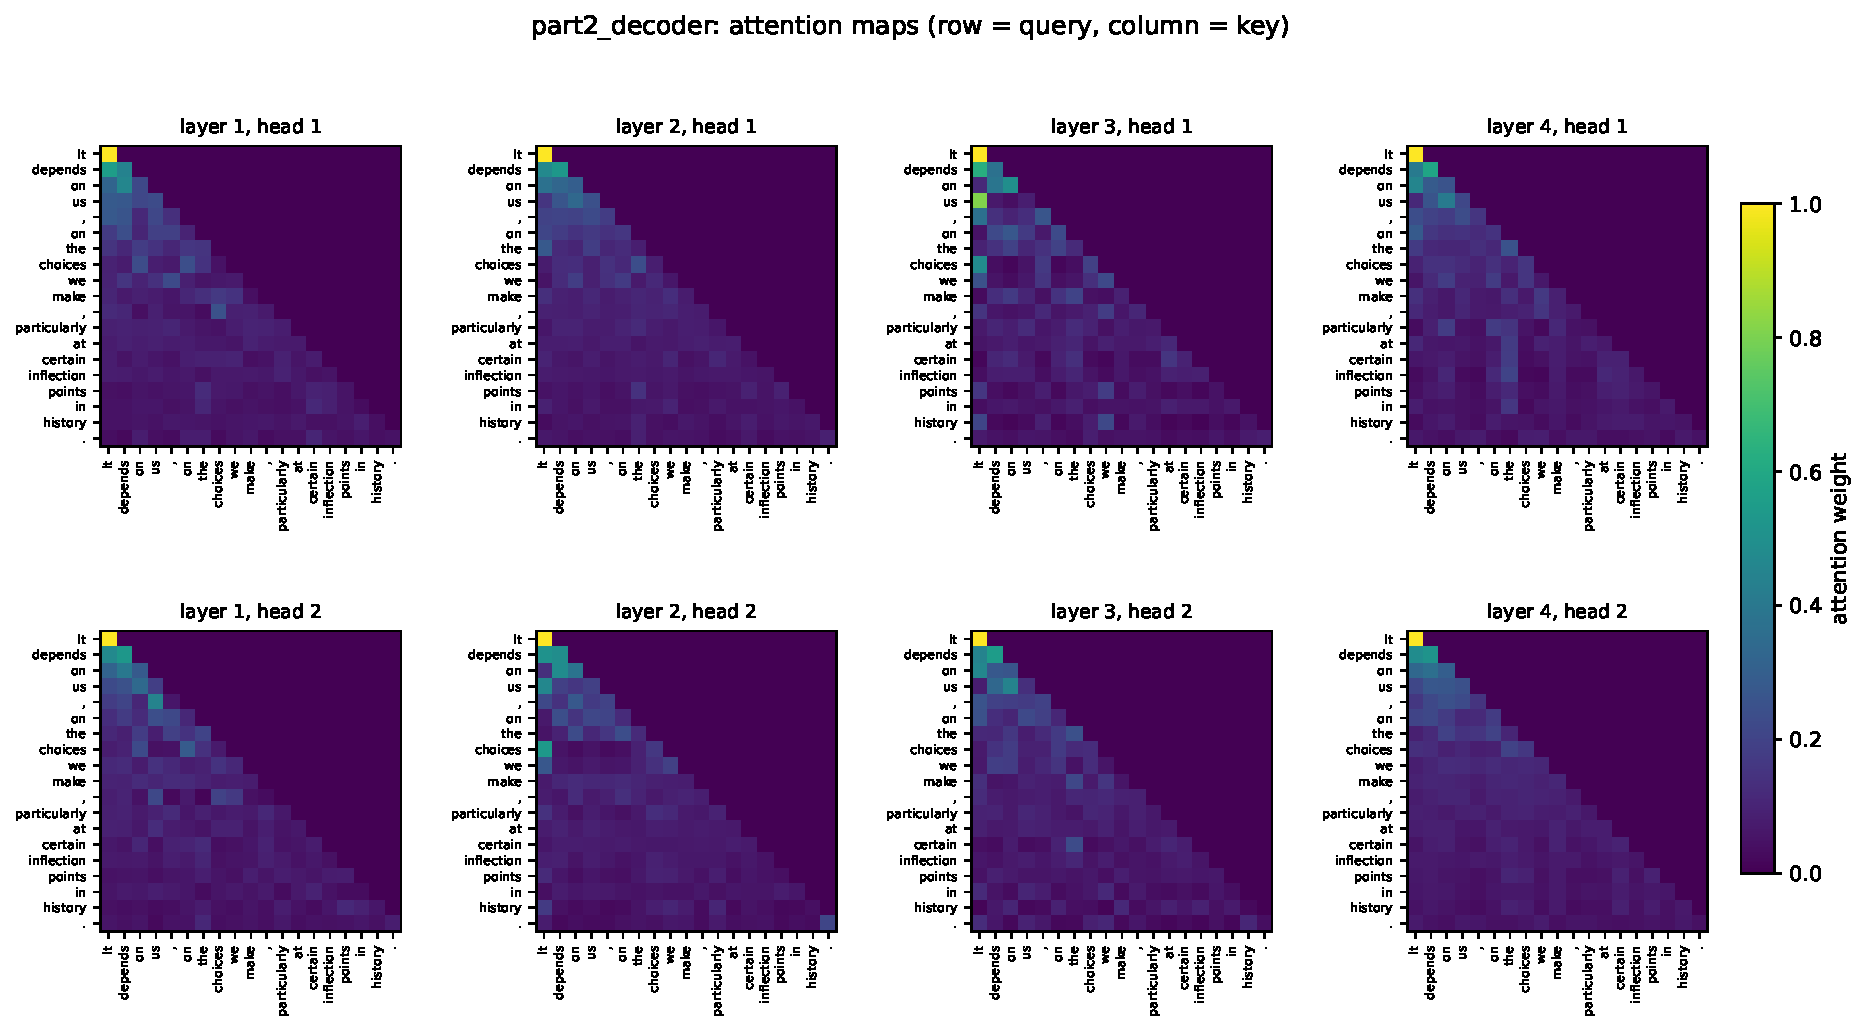
\includegraphics[width=0.82\linewidth, trim=0 0 0 40, clip]{figures/part2_decoder_attention_s1.pdf}
\caption{Decoder attention maps for the same sentence as Figure~\ref{fig:attn-enc} (rows are heads, columns are layers). Every map is lower-triangular because of the causal mask.}
\label{fig:attn-dec}
\end{figure}

\textbf{What the decoder maps show} (decoder columns of Table~\ref{tab:attn}):
\begin{itemize}
  \item \textbf{The decoder mostly averages over its past.} Below the diagonal the maps are mostly diffuse. Over the whole Obama test file every head has normalized entropy between 0.928 and 0.988. The weight on the first token (about 0.10) is what uniform attention would give, so the bright first column is just the effect of the early rows.
  \item \textbf{A few heads show mild, local preferences.} Layer 1 head 1 favours the previous word (0.113 vs 0.099 for uniform), which helps predict the next word. Layer 3 head 1 and layer 2 head 2 are the most selective (entropy 0.928 and 0.939, largest weight about 0.20). In Figure~\ref{fig:attn-dec}, layer 3 head 1 sends much of the weight of \textit{us} and \textit{choices} back to the sentence-initial \textit{It}.
  \item \textbf{The encoder is even closer to uniform} (entropy 0.939--1.000 vs 0.928--0.988). The decoder needs some position-specific attention, such as the previous word, to predict the next one. The encoder is trained only through the sentence mean (Section~1.4). With 4 small layers and little data, neither model learns sharp, syntax-like heads.
\end{itemize}

\subsection*{2.4\quad Evaluation}

\textbf{Method.} Perplexity is $\exp$ of the mean cross-entropy per token. I evaluate it on whole files, cut into non-overlapping 32-token windows, so every token is predicted exactly once with 0--31 tokens of context. The starter \code{compute\_perplexity} referenced an undefined variable; my version averages the loss over all predicted tokens.

\begin{figure}[H]
\centering
\begin{minipage}[c]{0.42\linewidth}
\centering
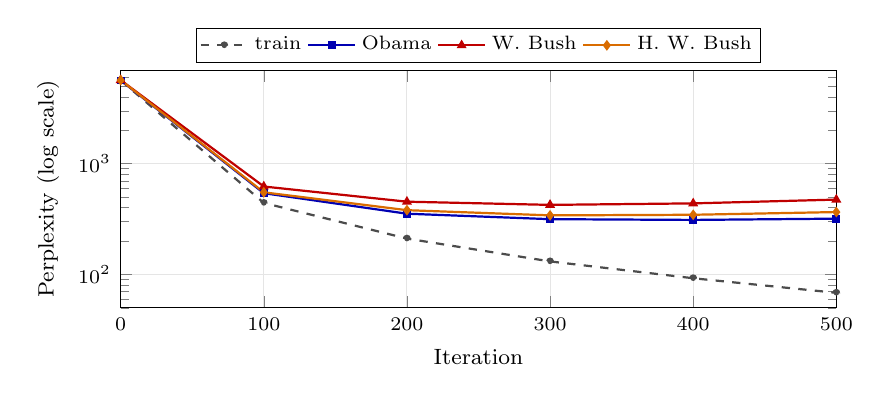
\begin{tikzpicture}
\begin{semilogyaxis}[rpt, width=0.88\linewidth,
  xlabel={Iteration}, ylabel={Perplexity (log scale)},
  xmin=0, xmax=500, ymin=50, ymax=7000, xtick={0,100,...,500},
  legend style={at={(0.5,1.03)}, anchor=south}, legend columns=4]
\addplot[thick, dashed, color=gray!60!black, mark=*, mark size=1pt] coordinates {
(0,5659.73)(100,442.25)(200,210.78)(300,131.15)(400,92.42)(500,68.27)};
\addlegendentry{train}
\addplot[thick, color=blue!70!black, mark=square*, mark size=1pt] coordinates {
(0,5650.19)(100,541.75)(200,353.64)(300,315.64)(400,310.74)(500,318.98)};
\addlegendentry{Obama}
\addplot[thick, color=red!75!black, mark=triangle*, mark size=1.3pt] coordinates {
(0,5679.53)(100,622.39)(200,453.92)(300,424.81)(400,438.22)(500,474.10)};
\addlegendentry{W.\ Bush}
\addplot[thick, color=orange!85!black, mark=diamond*, mark size=1.3pt] coordinates {
(0,5680.13)(100,551.60)(200,380.52)(300,341.59)(400,345.87)(500,365.94)};
\addlegendentry{H.\ W.\ Bush}
\end{semilogyaxis}
\end{tikzpicture}
\captionof{figure}{Perplexity during pretraining (seed 42).}
\label{fig:p2}
\end{minipage}\hfill
\begin{minipage}[c]{0.55\linewidth}
\centering
\footnotesize
\setlength{\tabcolsep}{2.6pt}
\captionof{table}{Perplexity every 100 iterations (seed 42), the mean $\pm$ s.d.\ of the final values over seeds 42, 1, 2, 3, and the final values with PyTorch's default initialization.}
\label{tab:p2}
\begin{tabular}{@{}l r r r r@{}}
\toprule
Iteration & Train & Obama & W.\ Bush & H.\ W.\ Bush \\
\midrule
0   & 5{,}660 & 5{,}650 & 5{,}680 & 5{,}680 \\
100 & 442.3 & 541.8 & 622.4 & 551.6 \\
200 & 210.8 & 353.6 & 453.9 & 380.5 \\
300 & 131.2 & 315.6 & \textbf{424.8} & \textbf{341.6} \\
400 & 92.4  & \textbf{310.7} & 438.2 & 345.9 \\
500 (final) & \textbf{68.3} & 319.0 & 474.1 & 365.9 \\
\midrule
Final, 4 seeds & 67.3 $\pm$ 0.7 & 322.5 $\pm$ 3.8 & 469.2 $\pm$ 4.7 & 367.4 $\pm$ 6.1 \\
Final, PyTorch init & 171.0 & 382.2 & 508.2 & 409.7 \\
\bottomrule
\end{tabular}
\end{minipage}
\end{figure}

\textbf{Results.}
\begin{itemize}
  \item \textbf{Initial perplexity is a sanity check.} At iteration 0 every perplexity is about 5{,}650, close to the vocabulary size of 5{,}634, as expected for a model that predicts nearly uniformly.
  \item \textbf{Final test perplexities are 319.0 (Obama), 474.1 (W.\ Bush) and 365.9 (H.\ W.\ Bush)}, in the expected 300s and 400s. The ordering Obama $<$ H.\ W.\ Bush $<$ W.\ Bush holds at every evaluation point after training starts, and for every seed. The seed-to-seed spread (s.d.\ 3.8--6.1) is far smaller than the gaps between politicians (45--147).
  \item \textbf{The model starts to overfit after 300--400 iterations.} Training perplexity keeps falling (131 $\rightarrow$ 68 from iteration 300 to 500), but test perplexity bottoms out and then rises: W.\ Bush 425 $\rightarrow$ 474, H.\ W.\ Bush 342 $\rightarrow$ 366, Obama 311 $\rightarrow$ 319.
\end{itemize}

\textbf{Why the three politicians get different perplexities.} The differences come mainly from \textbf{how much of each politician's language the model saw during pretraining} (Table~\ref{tab:data}).

\begin{table}[H]
\centering
\footnotesize
\setlength{\tabcolsep}{4pt}
\caption{How much each test set resembles the LM training text (\code{python data\_stats.py}). Speaker counts come from matching the 1{,}553 lines of \code{train\_LM.txt} against the labeled classification files. ``Unseen'' words are in the vocabulary (it also includes \code{train\_CLS.tsv}) but never occur in \code{train\_LM.txt}.}
\label{tab:data}
\begin{tabular}{@{}l ccc@{}}
\toprule
& Obama & W.\ Bush & H.\ W.\ Bush \\
\midrule
Lines of \code{train\_LM.txt} attributed to the speaker (516 unmatched) & \textbf{612} & \textbf{0} & 425 \\
Test words never seen in \code{train\_LM.txt} & 7.35\% & \textbf{9.41\%} & 8.23\% \\
Test bigrams that also occur in \code{train\_LM.txt} & 53.2\% & \textbf{45.7\%} & 51.5\% \\
Unigram model perplexity (add-one, trained on \code{train\_LM.txt}) & 655.5 & \textbf{735.1} & 663.0 \\
\code{<unk>} rate / test tokens & 1.93\% / 5{,}549 & 2.13\% / 4{,}795 & 2.13\% / 4{,}778 \\
\midrule
Decoder test perplexity (seed 42) & 319.0 & \textbf{474.1} & 365.9 \\
\bottomrule
\end{tabular}
\end{table}

\begin{itemize}
  \item \textbf{W.\ Bush appears to be missing from the training text.} Of the 1{,}037 training lines that can be attributed to a speaker, 612 are Obama's, 425 are H.\ W.\ Bush's and none are W.\ Bush's; the other 516 lines cannot be attributed this way. Obama has the most training text and the lowest perplexity (319). H.\ W.\ Bush has less and is in between (366). W.\ Bush has the least overlap and the highest perplexity (474).
  \item \textbf{Less overlap means more surprising words and phrases.} W.\ Bush's test set has the most words the decoder never saw as training targets (9.4\%) and the fewest familiar bigrams (45.7\%). The output layer gives unseen words very low probability, because during training their logits are only ever pushed down. \code{main.py} measures what they cost:
  \begin{itemize}
    \item about 12.8--12.9 nats each, versus 5.2--5.5 for the other tokens;
    \item 7.4\% / 9.4\% / 8.2\% of the tokens (Obama / W.\ Bush / H.\ W.\ Bush), but 16.5\% / 19.7\% / 17.8\% of the total test loss.
  \end{itemize}
  The familiar tokens show the same ranking: their mean loss is 5.20 / 5.46 / 5.29, or perplexity 181 / 235 / 198. So unseen words widen the gaps, but the model also predicts W.\ Bush's familiar words less well.
  \item \textbf{A unigram model gives the same ranking.} Even this baseline, which ignores context entirely, ranks the sets Obama $<$ H.\ W.\ Bush $<$ W.\ Bush (656 / 663 / 735). So the ranking reflects how far each speaker's vocabulary and topics are from the training text, not a quirk of the Transformer.
  \item \textbf{The Transformer amplifies the gaps.} Its gain over the unigram baseline is largest for Obama (perplexity divided by 2.05), then H.\ W.\ Bush (1.81) and W.\ Bush (1.55). It has learned phrase-level patterns that transfer best to the speakers it was trained on.
  \item \textbf{Overfitting hits the unseen speaker hardest.} After iteration 300, W.\ Bush's perplexity rises the most (+49, against +24 for H.\ W.\ Bush and +3 for Obama), as the model specializes to the two speakers in its training text.
  \item \textbf{Other explanations are ruled out.} The \code{<unk>} rates are nearly equal (1.9--2.1\%), and almost no test lines appear verbatim in the training text (2, 0 and 2 of 250), so neither explains the differences.
\end{itemize}

\subsection*{Part 3 (rubric items 3--5): where to find each answer in Part B}

\begin{table}[H]
\centering
\footnotesize
\begin{tabular}{@{}l l l@{}}
\toprule
Gradescope item & Handout question & Notebook section (Part B) \\
\midrule
3.1 Why checkpoints (2 pts) & 3.1, question 1 & 3.1.1 Why checkpoints? --- Answer 3.1.1 \\
3.2 Data (2 pts) & 3.1, question 2 & 3.1.2 Data --- Answer 3.1.2 \\
4.1 Watch a prediction form (13 pts) & 3.2.1 & 3.2.1 --- grids (i), (ii), accuracy curve (iii), Answer 3.2.1 \\
4.2 Across training (13 pts) & 3.2.2 & 3.2.2 --- four-checkpoint plot, Answer 3.2.2 \\
5 Transplanting layers across time (20 pts) & 3.3 & 3.3 --- heatmap, extra plots and experiment, Answer 3.3 \\
\bottomrule
\end{tabular}
\end{table}

\paragraph{Use of AI tools.} I used Claude (Anthropic)~\cite{claude} to help write and debug the code and to draft this report.

\begin{thebibliography}{3}
\setlength{\itemsep}{1pt}
\small
\bibitem{vaswani} Ashish Vaswani, Noam Shazeer, Niki Parmar, Jakob Uszkoreit, Llion Jones, Aidan N.\ Gomez, {\L}ukasz Kaiser, and Illia Polosukhin. Attention is all you need. In \emph{NeurIPS}, 2017.
\bibitem{karpathy} Andrej Karpathy. Let's build GPT: from scratch, in code, spelled out. \url{https://www.youtube.com/watch?v=kCc8FmEb1nY}, 2023.
\bibitem{claude} Anthropic. Claude. Large language model assistant, \url{https://claude.ai}, 2026.
\end{thebibliography}

\end{document}
